\documentclass[10pt,twoside]{pnas-new}
% Use the lineno option to display guide line numbers if required.

\templatetype{pnasmathematics} % Choose template 
% {pnasresearcharticle} = Template for a two-column research article
% {pnasmathematics} = Template for a one-column mathematics article
% {pnasinvited} = Template for a PNAS invited submission

%remove watermark
\setboolean{displaywatermark}{false}

\title{Topological  Fractal  Dimension  of  Networks  of Protein–Protein  Interaction  Networks}
%PNAS LaTeX Template for preparing single-column mathematics articles on Overleaf
% Use letters for affiliations, numbers to show equal authorship (if applicable) and to indicate the corresponding author
\author[a]{Georgios Kalantzis}
\author[a]{Andrei Stoica} 

\affil[a]{SABS, DTC}

% Please give the surname of the lead author for the running footer
%\leadauthor{Lead author last name} 

% Please add here a significance statement to explain the relevance of your work
\significancestatement{Authors must submit a 120-word maximum statement about the significance of their research paper written at a level understandable to an undergraduate educated scientist outside their field of speciality. The primary goal of the Significance Statement is to explain the relevance of the work in broad context to a broad readership. The Significance Statement appears in the paper itself and is required for all research papers.}

% Please include corresponding author, author contribution and author declaration information
%\authorcontributions{Please provide details of author contributions here.}
%\authordeclaration{Please declare any conflict of interest here.}
%\equalauthors{\textsuperscript{1}A.O.(Author One) and A.T. (Author Two) contributed equally to this work (remove if not applicable).}
%\correspondingauthor{\textsuperscript{2}To whom correspondence should be addressed. E-mail: author.two\@email.com}

% Keywords are not mandatory, but authors are strongly encouraged to provide them. If provided, please include two to five keywords, separated by the pipe symbol, e.g:
\keywords{PPIN $|$ NetworkX $|$ BioGrid $|$ Network Science $|$ Centrality Measures} 

\begin{abstract}
Please provide an abstract of no more than 250 words in a single paragraph. Abstracts should explain to the general reader the major contributions of the article. References in the abstract must be cited in full within the abstract itself and cited in the text.
\end{abstract}

\dates{This manuscript was compiled on \today}
%\doi{\url{www.pnas.org/cgi/doi/10.1073/pnas.XXXXXXXXXX}}

\begin{document}

\maketitle
\thispagestyle{firststyle}
\ifthenelse{\boolean{shortarticle}}{\ifthenelse{\boolean{singlecolumn}}{\abscontentformatted}{\abscontent}}{}

\section{Introduction \& Prerequisites}
Networks are representations of real systems where individual units are modelled as nodes and interactions between these units as links. Formally speaking, this corresponds to a graph $\mathcal{G} = (\mathcal{V},\mathcal{E})$, with $\mathcal{V}$ and $\mathcal{E}$ standing for the set of nodes and edges respectively. However, nodes can be anything, ranging from regions of the human brain to electrical power plants. As a result, the study of networks pervades all of science, from neurobiology to statistical physics~\cite{strogatz2001exploring}.  

The set of nodes $\mathcal{V}$ has usually a finite number of elements. Links can be undirected or directed, unweighted or weighted. When dealing with undirected edges, a link can be defined as a pair of nodes $(u,v)$; in directed graphs $(u,v)$ and $(v,u)$ correspond to different edges. In the case of weighted networks, links are also assigned with a real number characterising the importance of the association.

There are two main ways for representing networks, namely lists and adjacency matrices. Let $\mathbf{A}$ be the adjacency matrix of graph  $\mathcal{G}$ containing $n$ nodes. Then $\mathbf{A}$ is of size $n\times n$ and element $A_{ij}$ is $1$ if nodes $i,j$ are connected, otherwise, $A_{ij}=0$. In weighted networks non-zero elements of $\mathbf{A}$ are equal to the weights of edges. Moreover, real complex networks, although might contain thousands of nodes, are usually sparse in regards of edges and can be represented by sparse matrices which are special data structures.

After defining nodes and edges, the next important term is that of node-degree. The degree $k_i$ of node $i$ is defined as the number of edges linked to $i$. In directed graphs, the degree of a node might be discriminated in in-degree and out-degree, depending on whether the edges ending to or start from $i$ are counted. For undirected networks, the degree can be computed by
\[ k_i = \sum_{j=1}^{n}A_{ij} = \mathbf{e}_i^\top ( \mathbf{A} \cdot \mathbf{e} ), \]
where  $\mathbf{e}$ stands for a column-vector full of ones and $\mathbf{e}_i$ has zeros everywhere except element $i$ which is one. In other words, the product $ \mathbf{A} \cdot \mathbf{e} $ gives the degree for every node. These are some simple indicators showing why adjacency matrices are important: they connect Network Science with Linear Algebra.

Graphs are very attractive tools to biological and medical research applications, since they can use for description of many mechanisms or interactions, for instance metabolic or cell signalling networks. Another important direction are the so-called Protein-Protein Interaction Networks (which will be denoted as PPIN), which represent physical contacts between proteins within a cell. In brief, 
proteins are macromolecules, consisting of one or more long chains of amino acid residues, which perform a vast array of functions within organisms, including catalysing metabolic reactions, DNA replication, responding to stimuli, providing structure to cells and organisms, and transporting molecules from one location to another. Usually, the aforementioned procedures incorporate the cascade of many proteins, resulting in networks of interactions.

PPINs are characterised by three notable properties. First of all, PPINs show a small world effect meaning that there is great connectivity between proteins. More typically, the diameter (the maximum number of steps separating any two nodes) of such networks is small, regardless the number of nodes or edges. Such strong connectivity has important biological consequences, since it allows for an efficient and quick flow of signals within the network~\cite{PPINtrain}.

Moreover, PPINs are scale-free. This class of networks can describe a variety of complex systems where some nodes have a tremendous number edges (hubs), whereas most nodes have only a few~\cite{barabasi2003scale}. In this sense, the network appears to have no scale which provides important features. For instance, scale-free networks are very robust and stable since small perturbations have low effect. Furthermore, hubs in cancer-linked networks could be used for targeted attacks in drug discovery.

Finally, another crucial characteristic of PPINs is their modularity. The transitivity or clustering coefficient of a network is a measure of the tendency of the nodes to cluster together. High transitivity means that the network contains communities or groups of nodes that are densely connected internally. Generally speaking, structure always affects function~\cite{strogatz2001exploring}. In biological networks particularly, finding these communities is very important, because they can reflect functional modules and protein complexes.

However, PPINs are not real but correspond to actual biological networks and occur after experimental procedures. As a result, data might contain noise and some observations can be less reliable since the record of molecular interactions is occasionally incomplete or patchy.

\section{Construction of PPIN and Analysis}
\label{sec:2-task1}
There are various software packages or programmatic methods available to build and analyse networks. Throughout this project we work mainly with \PY and the \textsc{NetworkX} module. Furthermore, there are a lot of sources from which you can obtain and integrate PPI data, other than creating new experimental results. Current databases are distinguished in primary or predicting, depending on whether they just provide evidence or combine other resources for prediction. For the aims of this project we will be working with data from \textsc{BioGrid}, which is a primary curated biological database of protein-protein, genetic or chemical interactions as well as post-translational modifications.

\subsection{Hands-on \textsc{BioGrid} \& \NX }

PPINs can be created from edge-lists, which are text files containing rows of the form ``$\text{ID}_A - \text{ID}_B$''. The latter correspond to distinctive labels of nodes which can also be used as reference  to other information sources. After loading an edge-file, \NX  can initialise a graph with the provided edges.

In particular, we are using the dataset $\texttt{BIOGRID-ORGANISM-3.5.165.tab2.zip}$, offered freely in the \BGRD repository. This dataset contains information on protein interactions for $66$ organisms, stored in \texttt{Tab-2} format. Judging from the size of files, we can safely conclude that \textit{Saccharomyces Cerevisiae, Homo Sapiens} and \textit{Escherichia Coli K12} type W3110 have the largest numbers of protein interactions. 

\begin{wrapfigure}{r}{0.5\textwidth}
	\vspace{-25pt}
    \hspace{-80pt}
	%\centering
    \flushleft
	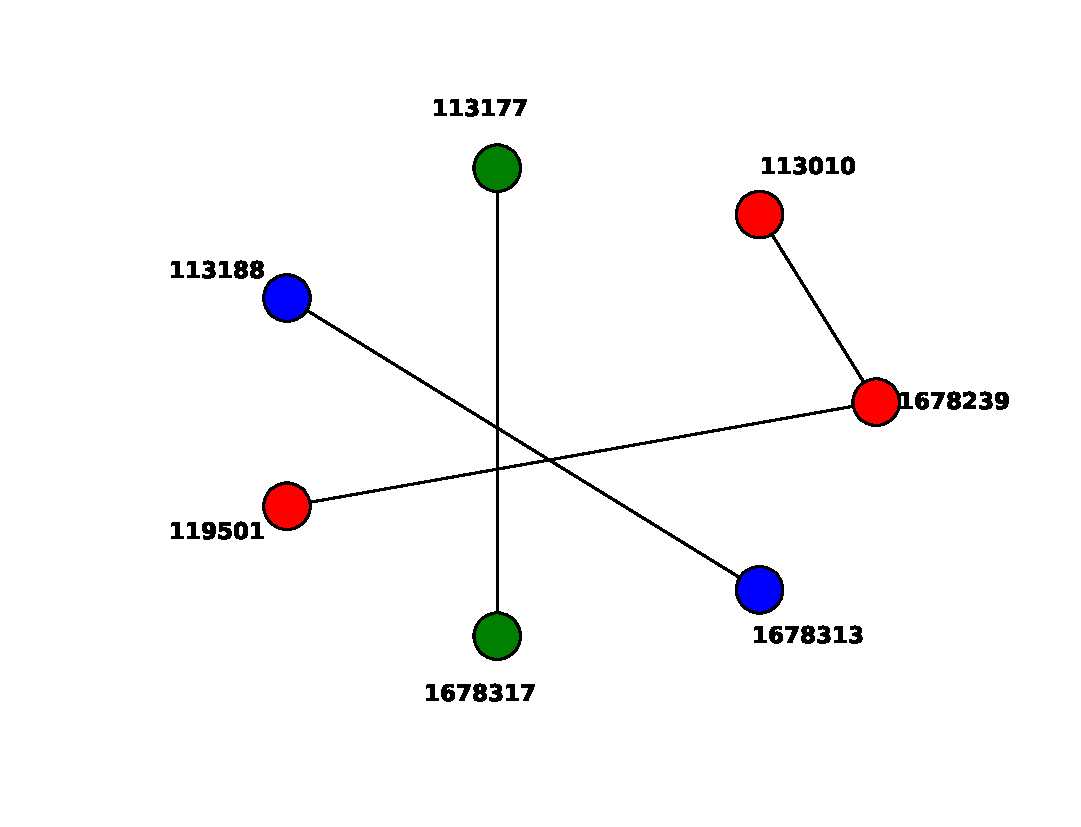
\includegraphics[width=.99\linewidth]{Graphics/Human_Herpesvirus_6Bgraph.eps}
	\caption{A simple PPIN, the one of \textit{Human Herpesvirus 6B}.}
	\label{fig:examplePPIN}
    \vspace{-10pt}
\end{wrapfigure}

\subsubsection*{An Example} Let us focus on \textit{Human Herpesvirus 6B}. After opening this file with a spreadsheet program we can easily observe that the first line (header) contains the labels of columns, followed by four lines with protein-protein interactions. What is more, there are $7$ nodes in total, divided in three components with the largest containing $3$ nodes. This PPIN is depicted in Figure~\ref{fig:examplePPIN} as visualized by \NX. 

In order to create a PPIN, what we need is a type for protein labeling. Given this dataset, there are up to three different ways, for example by using information from \textit{Entrez} database or official symbols. We chose to work with the \textsc{BioGrid} IDs since these labels are numerical and they reference directly to the online repository. 

One drawback of \BGRD is the existence of some noise in the data. By this we mean multiple copies of the same interaction, which corresponds to parallel edges, or even self-loops. In order to remove such entries we used \PY's set datatype which is very efficient. Another part of pre-processing involved a re-labeling of nodes in order to construct necessary tables and arrays easier later on. To make this more helpful, we also saved a dictionary with correspondences between new and initial labels for every organism.  These steps are implemented in script \texttt{ParseBioGridFiles.py} and the functions therein.

\subsection{Basic Information \& Illustration of PPINs}
%\def\rownumber{} % hack for re-starting row-counter (and skip the header) 
\begin{table}[h] %[tbhp]
	\centering
	\caption{\textit{Appendix} - Basic Information about PPINs from \texttt{BioGrid 3.5.165 dataset}}
	\label{table:stats}
    \begin{tabular}{@{\makebox[2em][r]{\rownumber\space}} | lrrcccr}
		\textbf{Organism} & \textbf{\# Nodes} &  \textbf{\# Edges} & \textbf{Avg Degree} & \textbf{ConComps} & \textbf{Largest} & \textbf{Diam} %[0.5ex] 
        \gdef\rownumber{\stepcounter{magicrownumbers}\arabic{magicrownumbers}} \\
		\midrule
        $ Anopheles \ gambiae \ PEST $ & 2 & 1 & 1.00 & 1 & 1.000 & 1 \\ 
        $ Apis \ mellifera $ & 2 & 1 & 1.00 & 1 & 1.000 & 1 \\ 
        $ Arabidopsis \ thaliana \ Columbia $ & 9570 & 35242 & 7.37 & 78 & 0.981 & 12 \\ 
        $ Bacillus \ subtilis \ 168 $ & 2 & 1 & 1.00 & 1 & 1.000 & 1 \\ 
        $ Bos \ taurus $ & 437 & 405 & 1.85 & 73 & 0.162 & 15 \\ 
        $ Caenorhabditis \ elegans $ & 3938 & 7885 & 4.00 & 77 & 0.953 & 13 \\ 
        $ Candida \ albicans \ SC5314 $ & 713 & 860 & 2.41 & 30 & 0.893 & 12 \\ 
        $ Canis \ familiaris $ & 52 & 34 & 1.31 & 20 & 0.135 & 4 \\ 
        $ Cavia \ porcellus $ & 9 & 5 & 1.11 & 4 & 0.333 & 2 \\ 
        $ Chlamydomonas \ reinhardtii $ & 19 & 15 & 1.58 & 4 & 0.632 & 2 \\ 
        $ Chlorocebus \ sabaeus $ & 11 & 7 & 1.27 & 4 & 0.273 & 2 \\ 
        $ Cricetulus \ griseus $ & 32 & 24 & 1.50 & 8 & 0.500 & 3 \\ 
        $ Danio \ rerio $ & 245 & 250 & 2.04 & 37 & 0.404 & 8 \\ 
        $ Dictyostelium \ discoideum \ AX4 $ & 24 & 18 & 1.50 & 6 & 0.208 & 2 \\ 
        $ Drosophila \ melanogaster $ & 9191 & 54806 & 11.93 & 37 & 0.992 & 9 \\ 
        $ Emericella \ nidulans \ FGSC \ A4 $ & 64 & 62 & 1.94 & 6 & 0.703 & 2 \\ 
        $ Equus \ caballus $ & 4 & 2 & 1.00 & 2 & 0.500 & 1 \\ 
        $ Escherichia \ coli \ K12 $ & 2 & 1 & 1.00 & 1 & 1.000 & 1 \\ 
        $ Escherichia \ coli \ K12 \ MC4100 \ BW2952 $ & 10 & 8 & 1.60 & 2 & 0.800 & 6 \\ 
        $ Escherichia \ coli \ K12 \ MG1655 $ & 146 & 127 & 1.74 & 21 & 0.623 & 3 \\ 
        $ Escherichia \ coli \ K12 \ W3110 $ & 4063 & 181620 & 89.40 & 1 & 1.000 & 5 \\ 
        $ Gallus \ gallus $ & 391 & 417 & 2.13 & 42 & 0.588 & 9 \\ 
        $ Glycine \ max $ & 44 & 39 & 1.77 & 7 & 0.318 & 2 \\ 
        $ Hepatitus \ C \ Virus $ & 131 & 129 & 1.97 & 2 & 0.985 & 2 \\ 
        $ Homo \ sapiens $ & 22826 & 318912 & 27.94 & 14 & 0.999 & 9 \\ 
        $ Human \ Herpesvirus \ 1 $ & 174 & 194 & 2.23 & 1 & 1.000 & 8 \\ 
        $ Human \ Herpesvirus \ 2 $ & 7 & 4 & 1.14 & 3 & 0.429 & 2 \\ 
        $ Human \ Herpesvirus \ 3 $ & 4 & 2 & 1.00 & 2 & 0.500 & 1 \\ 
        $ Human \ Herpesvirus \ 4 $ & 240 & 235 & 1.96 & 7 & 0.771 & 8 \\ 
        $ Human \ Herpesvirus \ 5 $ & 91 & 79 & 1.74 & 12 & 0.385 & 4 \\ 
        $ Human \ Herpesvirus \ 6A $ & 11 & 7 & 1.27 & 4 & 0.364 & 2 \\ 
        $ Human \ Herpesvirus \ 6B $ & 7 & 4 & 1.14 & 3 & 0.429 & 2 \\ 
        $ Macaca \ mulatta $ & 15 & 12 & 1.60 & 3 & 0.733 & 2 \\ 
        $ Human \ Herpesvirus \ 7 $ & 2 & 1 & 1.00 & 1 & 1.000 & 1 \\ 
        $ Meleagris \ gallopavo $ & 2 & 1 & 1.00 & 1 & 1.000 & 1 \\ 
        $ Human \ Immunodeficiency \ Virus \ 1 $ & 1121 & 1299 & 2.32 & 1 & 1.000 & 5 \\ 
        $ Human \ Immunodeficiency \ Virus \ 2 $ & 16 & 12 & 1.50 & 4 & 0.500 & 4 \\ 
        $ Human \ papillomavirus \ 16 $ & 14 & 12 & 1.71 & 2 & 0.857 & 4 \\ 
        $ Mus \ musculus $ & 13003 & 38624 & 5.94 & 89 & 0.984 & 15 \\ 
        $ Neurospora \ crassa \ OR74A $ & 12 & 10 & 1.67 & 2 & 0.667 & 2 \\ 
        $ Mycobacterium \ tuberculosis \ H37Rv $ & 11 & 9 & 1.64 & 2 & 0.818 & 2 \\ 
        $ Nicotiana \ tomentosiformis $ & 2 & 1 & 1.00 & 1 & 1.000 & 1 \\ 
        $ Oryctolagus \ cuniculus $ & 283 & 271 & 1.92 & 33 & 0.502 & 9 \\ 
        $ Oryza \ sativa \ Japonica $ & 74 & 90 & 2.43 & 18 & 0.351 & 3 \\ 
        $ Pan \ troglodytes $ & 10 & 5 & 1.00 & 5 & 0.200 & 1 \\ 
        $ Ovis \ aries $ & 2 & 1 & 1.00 & 1 & 1.000 & 1 \\ 
        $ Pediculus \ humanus $ & 2 & 1 & 1.00 & 1 & 1.000 & 1 \\ 
        $ Plasmodium \ falciparum \ 3D7 $ & 1224 & 2445 & 4.00 & 23 & 0.963 & 10 \\ 
        $ Rattus \ norvegicus $ & 3713 & 5227 & 2.82 & 118 & 0.918 & 14 \\ 
        $ Ricinus \ communis $ & 3 & 2 & 1.33 & 1 & 1.000 & 2 \\ 
        $ Saccharomyces \ cerevisiae \ S288c $ & 7158 & 534073 & 149.22 & 1 & 1.000 & 6 \\ 
        $ Schizosaccharomyces \ pombe \ 972h $ & 4292 & 58217 & 27.13 & 7 & 0.997 & 8 \\ 
        $ Selaginella \ moellendorffii $ & 6 & 8 & 2.67 & 1 & 1.000 & 2 \\ 
        $ Simian \ Immunodeficiency \ Virus $ & 19 & 16 & 1.68 & 4 & 0.421 & 3 \\ 
        $ Simian \ Virus \ 40 $ & 6 & 5 & 1.67 & 1 & 1.000 & 2 \\ 
        $ Solanum \ lycopersicum $ & 45 & 96 & 4.27 & 7 & 0.467 & 4 \\ 
        $ Solanum \ tuberosum $ & 4 & 2 & 1.00 & 2 & 0.500 & 1 \\ 
        $ Sus \ scrofa $ & 94 & 79 & 1.68 & 23 & 0.234 & 5 \\ 
        $ Strongylocentrotus \ purpuratus $ & 17 & 16 & 1.88 & 1 & 1.000 & 2 \\ 
        $ Vaccinia \ Virus $ & 8 & 5 & 1.25 & 3 & 0.375 & 2 \\ 
        $ Tobacco \ Mosaic \ Virus $ & 3 & 2 & 1.33 & 1 & 1.000 & 2 \\ 
        $ Ustilago \ maydis \ 521 $ & 4 & 3 & 1.50 & 1 & 1.000 & 2 \\ 
        $ Xenopus \ laevis $ & 1128 & 1212 & 2.15 & 61 & 0.850 & 15 \\ 
        $ Vitis \ vinifera $ & 2 & 1 & 1.00 & 1 & 1.000 & 1 \\ 
        $ Zea \ mays $ & 21 & 11 & 1.05 & 10 & 0.143 & 2 \\ 
        $ Human \ Herpesvirus \ 8 $ & 714 & 687 & 1.92 & 45 & 0.529 & 12 \\ 
                %[1ex] 
		\bottomrule
    \end{tabular}
	%\addtabletext{nomenclature for the TSs refers to the numbered species in the table.}
\end{table}
The first step of the analysis was the calculation of some fundamental properties for each PPIN, i.e. number of nodes ($N$), number of edges ($M$), average degree of nodes, number of connected components, relative size of largest connected component (LGC) and diameter. The later is computed for the LGC, for disconnected cases.  All these are summarized in Table~\ref{table:stats} (\textit{Appendix}). 

Interestingly, the majority of small PPINs, i.e. those with only a few hundreds of nodes or less, show low connectivity. Two characteristic examples are \textit{Bos taurus} (cattle) or \textit{Danio rerio} (zebrafish) whose largest connected component contains $16\%$ and $40\%$, respectively, of the total nodes. Larger networks, on the contrary, show a very different behavior regarding connectivity; almost every PPIN containing thousands of nodes has a giant component containing more than $90\%$ of nodes. One such notable example is that of \textit{Human Immunodeficiency Virus 1}, which is fully connected, illustrated Figure~\ref{fig:HIV}. 

\begin{figure}
  \centering
  \vspace{-70pt}
  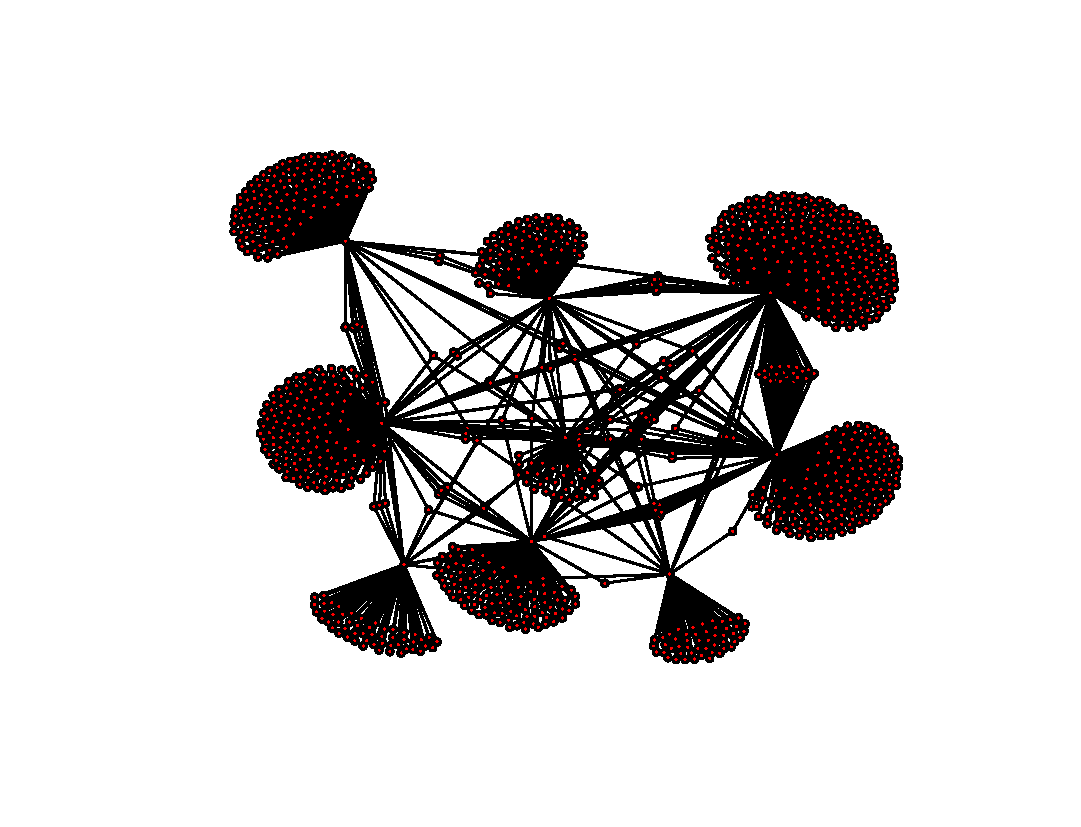
\includegraphics[width=.99\linewidth]{Graphics/Human_Immunodeficiency_Virus_1graph.eps}
  \vspace{-30pt}
  \caption{PPIN of \textit{Human Immunodeficiency Virus 1}.}
  \label{fig:HIV}
\end{figure}

\subsection{Centrality \& Important Proteins}
One of the most useful tasks in Network Science is the location of the most central or important nodes. This has always been of high importance in many scientific fields with a seminal work from Sociology aging more than six decades~\cite{katz1953new}. After the enormous expansion of World Wide Web and the need of finding meaningful websites efficiently, the field of Node Ranking has gained a lot of attention the last two decades \cite{langville2011google}. To date, there is a variety of algorithms that measure centrality in order to estimate the most important ones, each with specific advantages, but also drawbacks, regarding speed, accuracy and the need of resources.   

\NX, in particular, has a lot of built-in algorithms for node centrality, some of which we used for the analysis. First of all, \texttt{Degree Centrality} is by far an easy to compute measure and yet meaningful as it considers every direct interaction. \texttt{Katz Index} and \texttt{HITS} are algorithms that place emphasis on indirect connections. \texttt{PageRank} does also the same but in a more computationally efficient way as it incorporates many tools. The last measure we are using is \texttt{Closeness Centrality} which corresponds to the reciprocal of the average distance of a node to every other. A lot of PPINs are divided in connected components which would result in frailty when calculating closeness as some distances would be equal to infinity. To overcome this obstacle, closeness centrality is defined by an improved formula~\cite{wasserman1994social} as
\begin{equation}
	C(u) = \frac{n-1}{N-1} \frac{n - 1}{\sum_{v=1}^{n-1} d(v, u)},
\end{equation}
where n is the size of the related component and $d(u,v)$ is shortest path (i.e. the distance) between nodes $u$ and $v$. Calculating the aforementioned distances is a difficult task, however, since this is part of the next task in the project (see Section~\ref{sec:3-task2}), we implemented a new function that calculates the closeness centralities, given the distances (check function \texttt{MyCloseness} in \texttt{PPINutils.py} script). \texttt{PageRank} and \texttt{HITS} are implemented by \NX in an optimal way (\textit{scipy versions}) which, even for the largest PPINs needed only a few seconds of running time. \texttt{Katz}, on the other hand, requires the solution of a system of linear equations (or the inversion of a huge matrix otherwise), which is very time-consuming. We also tried to compute the \texttt{Betweenness Centrality} but without success, due to the high demand of processing resources.

We are now focusing on \textit{Homo sapiens}, a PPIN with $22826$ nodes, for the estimation of the most central proteins. On a typical DTC computer ($3.50$ GHz and $7.7$ GB of RAM), \texttt{PageRank} and \texttt{Degree Centrality} took less than two seconds to run and \texttt{HITS} required approximately ten seconds. Closeness centralities were computed in almost three minutes and, finally, \texttt{Katz} took more than $45$ minutes. Some of the resulting rankings seem to be consistent whereas other are dissimilar. For instance, \texttt{HITS} ``agrees'' with \texttt{PageRank} by $TODO$ counted by Spearmann's $\rho$ ranking coefficient. 

In order to select the most important nodes we do the following procedure: we select the top-$15$ ranked nodes by each of the five algorithms, create a list with all these $75$ elements and count the multiple occurrences. The most frequent proteins are reported in Table~\ref{tab:central} accompanied by the corresponding gene and protein function. 


\begin{table}[h]%[tbhp]
	\centering
	\caption{Top-5 Central Proteins in \textit{Homo Sapiens}}
	\begin{tabular}{cccl}
		Node Label & Protein & Gene & Function \\
		\midrule
		114030 & Cullin-3 & CUL3 & This protein plays a critical role in the polyubiquitination and subsequent degradation of specific protein substrates \\
		113164 & HMG20 &  UBC & It plays a key role in maintaining cellular ubiquitin levels under stress. Defects could lead to embryonic lethality. \\
		108309 & HuR & ELAVL1 & RNA-binding protein that binds to the 3'-UTR region of mRNAs and increases their stability \\
		113348 & Exportin-1 & XPO1 &  eukaryotic protein that mediates the nuclear export of proteins, rRNA, snRNA, and some mRNA. \\
		113010 & TP53 & TP53 & tumor suppressor protein containing transcriptional activation, DNA binding, and oligomerization domains.  \\
		%\[ 114030,\ 113164,\ 108309,\ 113348,\ 113010. \]
        \bottomrule
		\label{tab:central}
	\end{tabular}
\end{table}

\subsection{Degree Distributions}

We move to another interesting aspect of complex networks which concerns the distribution of degrees. Although many of the constructed PPINs are interesting, for the sake of clarity we focus mainly on those by \textit{Homo sapiens} and HIV. We present such information in Figures~\ref{fig:DD_Hs}-\ref{fig:DD_HIV}. In general, as was also mentioned in Section~\ref{SS:Intro}, most of the PPINs are scale-free since there are hubs that are connected with a large proportion of nodes and, on the same time, a lot of nodes have only a few edges. This behavior, which is explained by the fact that degree distributions of such networks usually follow a power-law \cite{barabasi2003scale}, can be observed by the histograms (left part of the following figures).  

\begin{figure}[h]
	\begin{minipage}{0.51\textwidth}
		%\flushleft
		%\centering
		%\vspace{0pt}
		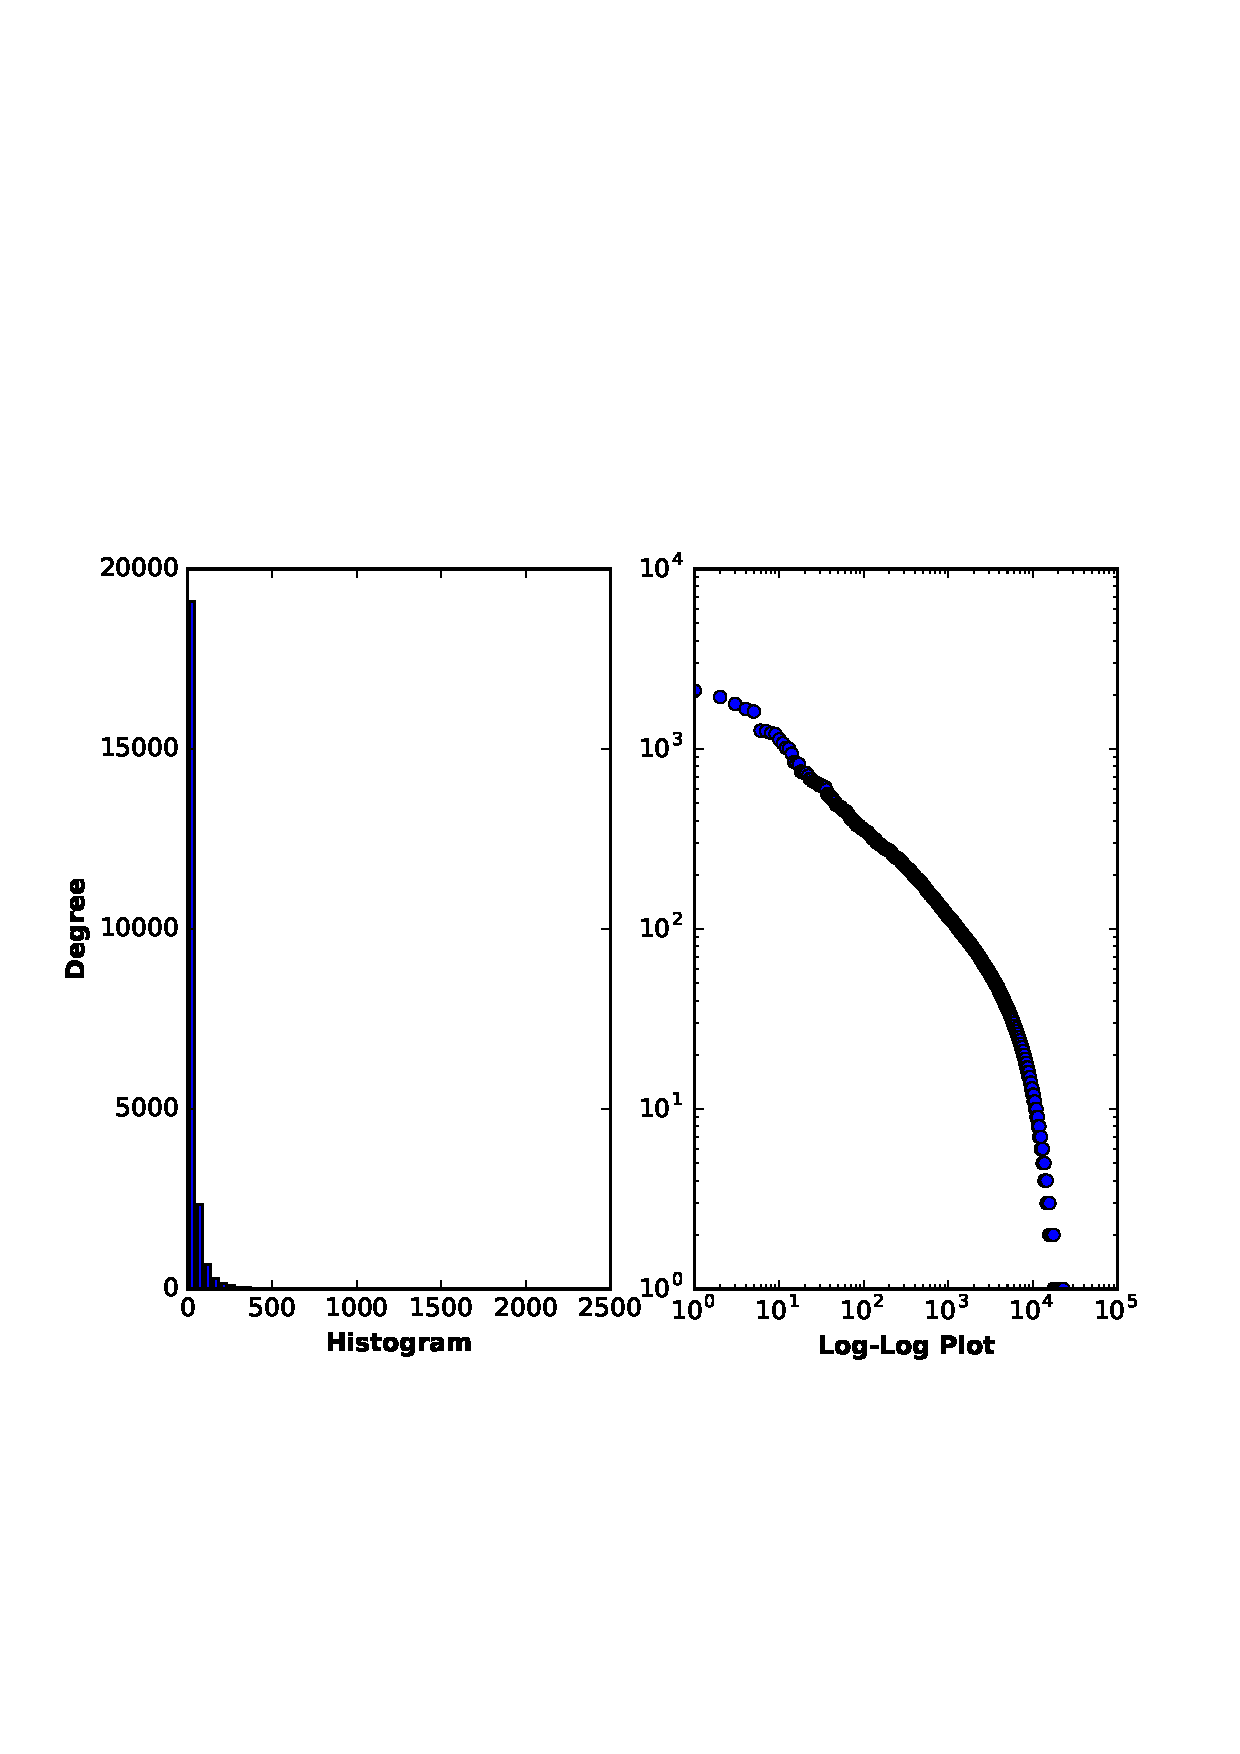
\includegraphics[width=\textwidth]{Graphics/Homo_sapiens-DD.png}
        \caption{Degree distribution in \textit{Homo sapiens}}
        \label{fig:DD_Hs}
	\end{minipage}
	%\hfill
	\begin{minipage}{0.51\textwidth}
		\flushleft
		%\vspace{10pt} % Hack for correct positioning
		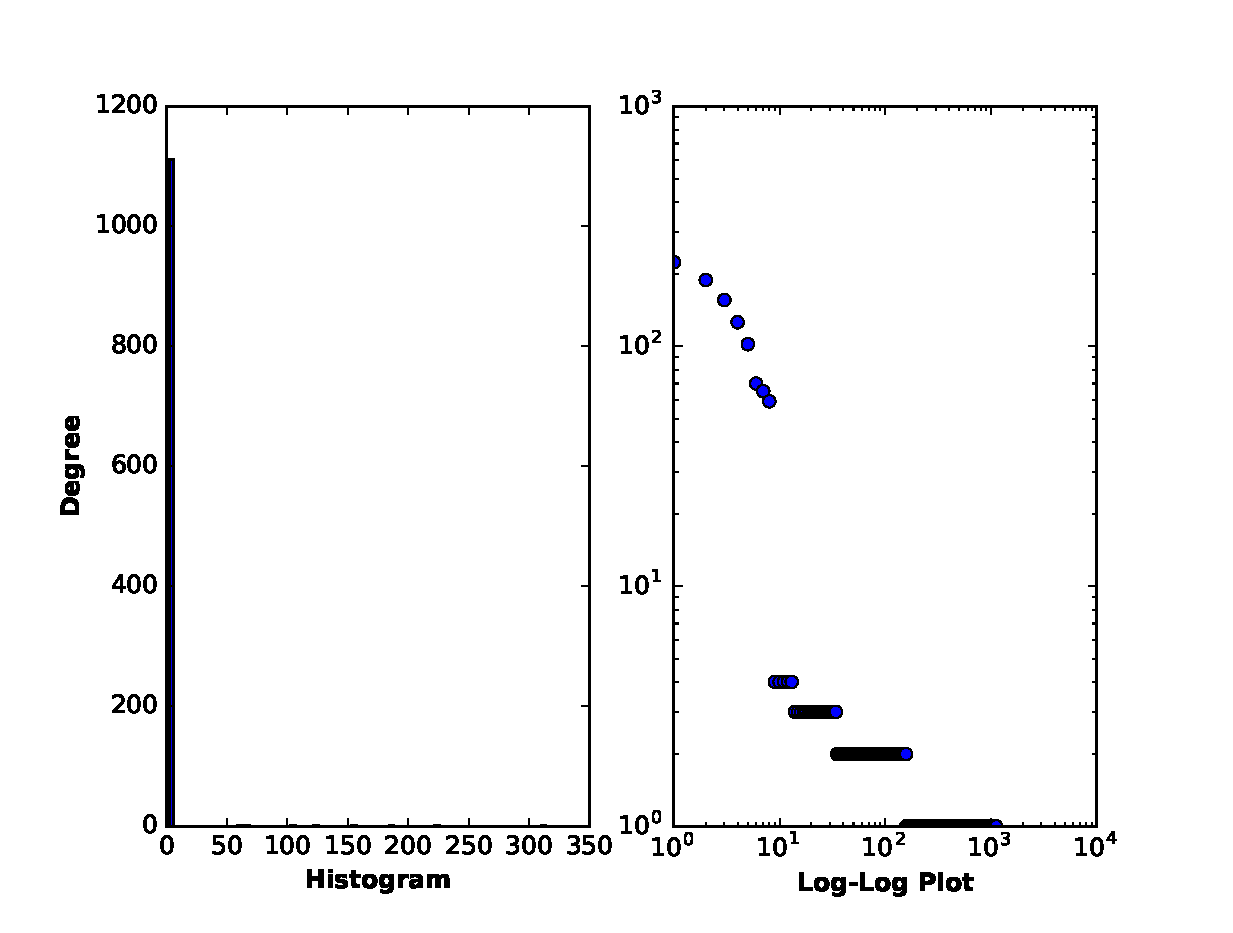
\includegraphics[width=\textwidth]{Graphics/Human_Immunodeficiency_Virus_1-DD}
		%\caption{{\small Graphical representation of }} 
        \caption{Degree distribution in \textit{HIV-1}}
		\label{fig:DD_HIV}
	\end{minipage}
\end{figure}

\subsection{Computational Complexity}
We are now investigating the time complexity for PPIN construction. There might be a variety of different ways  to study complexity but we measure the total time needed for loading an edge-file with \PY and adding the set of edges in a \NX graph. We assume that intermediate actions are the same for every organism and try to find a more abstract relationship between time ($T$) and size of graphs ($N or M$).

After measuring the time complexity for each of the  $66$ cases, we construct two plots in a logarithmic scale, as presented in Figures~\ref{fig:TimeVsEdges}-\ref{fig:TimeVsNodes}. We also plot a corresponding line after fitting a linear regression model. Despite the existence of some oscillations in small graphs, there seems to be a strong linear relationship between $T$ and $M$ and a less accurate linearity between $T$ and $N$. Speeding-up the construction of PPINs would require a deeper understanding of \PY's commands for file I/O. For instance, working with \texttt{Pandas} module instead of \texttt{csv.reader} gives a high advantage when constructing a graph from the scratch. On the other hand, we noticed that \texttt{csv.reader} was the only feasible way to read large files with node-distances. 

\begin{figure}[h]
	\begin{minipage}{0.51\textwidth}
		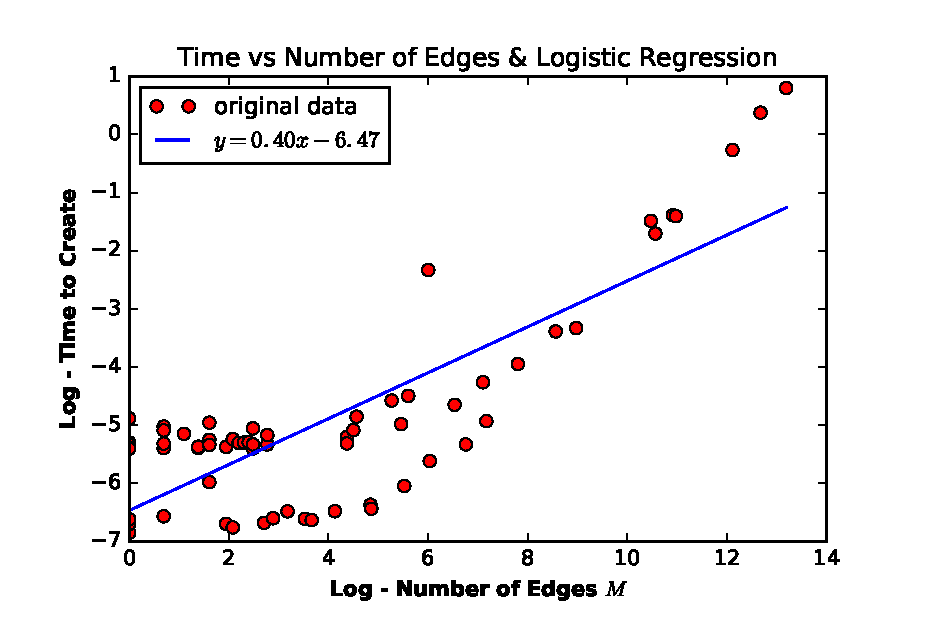
\includegraphics[width=\textwidth]{Graphics/TimeVsEdges.eps}
        \caption{Time vs Number of Edges}
        \label{fig:TimeVsEdges}
	\end{minipage}
	%\hfill
	\begin{minipage}{0.51\textwidth}
		\flushleft
		%\vspace{10pt} % Hack for correct positioning
		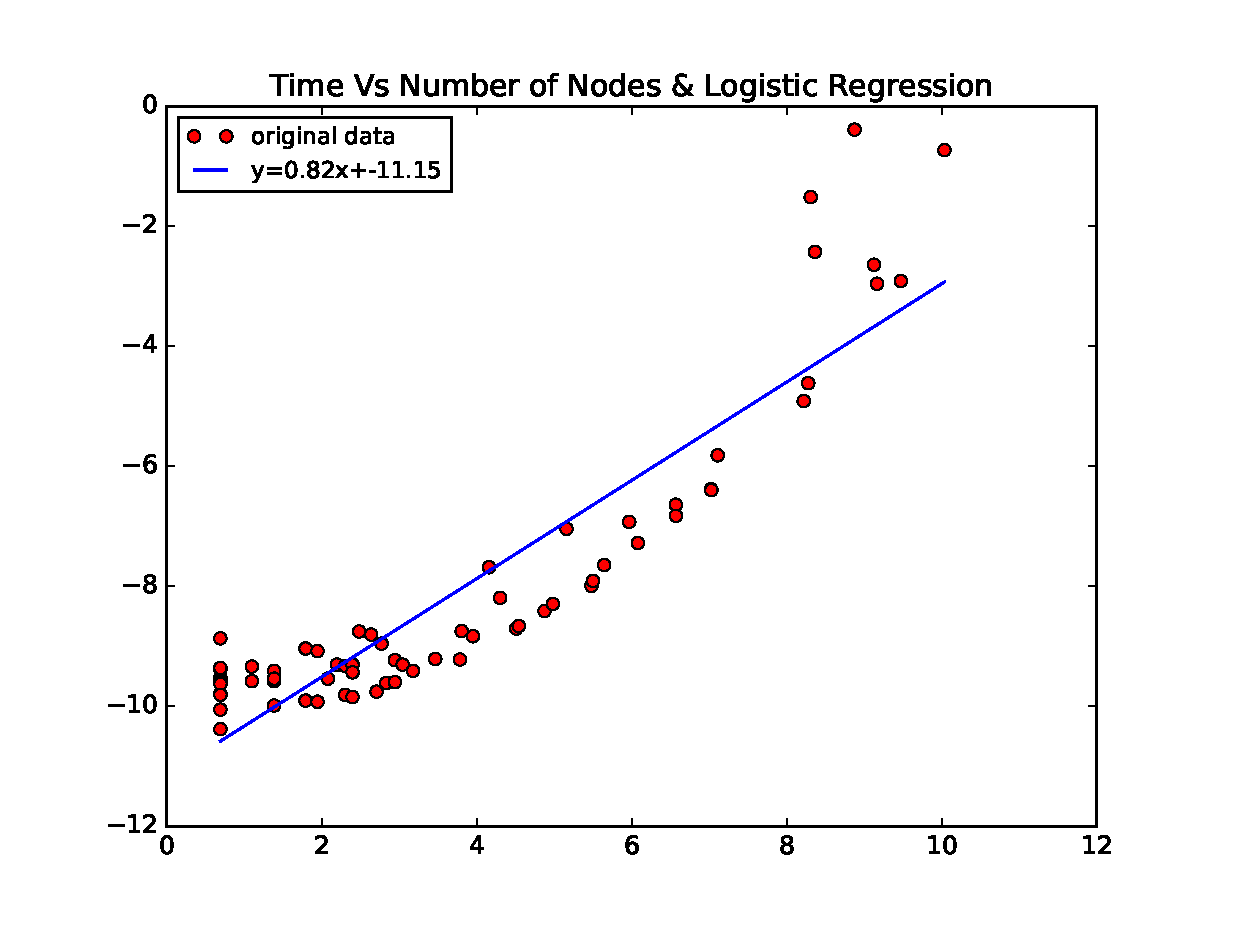
\includegraphics[width=\textwidth]{Graphics/TimeVsNodes.eps}
        \caption{Time vs Number of Nodes}
		\label{fig:TimeVsNodes}
	\end{minipage}
\end{figure}

%\subsection{Opt: The Development of PPINs} 

\section{Computing the Topological Fractal Dimension}
\label{sec:3-task2}
\subsection{The Box Counting Method}

Before we can introduce the concept of topological fractal dimension of a network, a preamble through the idea of box covering (originally due to Hausdorff) is necessary. Given a network $G$ and a box size $l_B$, a box covering of the network consists of an ensemble of disjoint boxes that together cover every node, with the property that the distance between any two nodes in each box is less than the given $l_B$ value. For any $l_B$ we define $N_B$ as the minimum number of boxes that are required for such a covering. It is thus clear that for $l_B=1$ we have that $N_B = N$, which is defined as the number of nodes. As we increase $l_B$, $N_B$ will correspondingly decrease, until a value of $1$ is obtained if the network is connected (or more generally, the minimal attainable $N$ will equal the number of connected components in the graph). We define the $l_B$ for which $N_B$ reaches its minimum as $l_B^{max}$

To identify the correct $N_B$ for a given $l_B$ in a reasonable amount of time, box covering algorithms have been developed. The problem of box covering is known to be NP-hard - that is, no algorithm will produce an exact solution in a reasonable amount of time. Therefore, existing algorithms only aim to optimally approximate $N_B$, rather than calculate it exactly.

For any given network, the $N_B$ and the $l_B$ values have been shown to satisfy a relation of the form:
\begin{equation} 
	N_B \sim l_B^{-d_B} \label{eq:powerlaw}
\end{equation}
The exponent $d_B$ is defined as the topological fractal dimension of the network. To determine it, first we employ a box covering algorithm to calculate the $N_B$. The method we chose was a greedy algorithm, as described in \cite{song2007how}, with the following steps:
\begin{enumerate}
\setlength{\itemsep}{-1pt}
	\item Initialize the network, numbering the nodes from 1 to N
	\item For all $l_B$ values, assign a box number of 0 for the first node.
	\item For $l_B$ values from 1 to $l_B^{max}$, repeat the following:
	\begin{itemize}
    \setlength{\itemsep}{-1pt}
    	\item For node i (starting at node 2) mark all box numbers where the distance between i and j is greater or equal than $l_B$ as unavailable 
        \item Select one box number from the remaining available ones for node i
        \item Increase i till it reaches N
        \item Increase $l_b$ till it reaches $l_b^{max}$
	\end{itemize}
\end{enumerate}


\subsection{Implementation}

This method necessitates information about the distances between every pair of nodes in the graph. This can be calculated as the algorithm is run (conveniently using the shortest path function from \NX) or alternatively pre-calculated before for every pair and stored in a matrix that will be read when the program that calculates the TFD starts. Due to speed constraints, we found the second approach to be preferable; as such, we wrote a C script to calculate the distance matrices for all $66$ different PPINs and we stored each one of then in a different file. Originally, the algorithm that we chose to calculate all the distances was Floyd-Warshall, due to simplicity of implementation. However, the speed of this dynamic programming algorithm proved insufficient for our needs, and we therefore switched to a breadth-first search (BFS) implementation, again done in C. The speed of computations was now satisfactory, and we managed to compute all the distances in our PPINs and then integrate them into the \PY program in order to calculate the number of boxes.

\subsection{Testing the Method}

The same \PY program was then used to calculate the TFD. To that direction, we rewrite Eq. \ref{eq:powerlaw} using a constant of proportionality $C$, then we take natural logarithms and rewrite everything in matrix form, forming a system of linear equations, as follows:

\begin{equation} \begin{bmatrix}
  \log N_1 \\
  \log N_2 \\
  \vdots \\
  \log N_{l_B^{max}} \\
\end{bmatrix} = \begin{bmatrix}
  1 & -\log l_1 \\
  1 & -\log l_2 \\
  \vdots & \vdots  \\
  1 & -\log l_B^{max} \\
\end{bmatrix}
\begin{bmatrix}
  \log C & d \\
\end{bmatrix}
\end{equation}

We solved for $C$ and $d$ using the linear least squares method from \PY's \textit{scipy} library. Before proceeding with the calculation on PPINs, we tested this greedy algorithm on synthetic networks. Three types of networks were considered: simple path graphs, lattice graphs and Erdos-Renyi graphs. In the path graph, where all the edges are between nodes with consecutive indices, we found that the value of the TFD seems to stabilize around 0.85 as we increase the number of nodes N. The theoretical predicted value was approximately 1, and the differences between it and the calculated value are likely to be due to the simplifying assumptions employed in order to find the theoretical value (detailed upon in the next section).

Regarding the lattice graph, where nodes form a grid, the expected value was 2. Our algorithm would obtain values as small as 1.2 for some of the smallest lattice graphs (e.g.$n=3$), but it would continuously increase and eventually reach a plateau around 2.35 (obtained for very large lattice graphs, with $n>230000$). The discrepancy between 2.35 and 2 is partly due to the fact that on lattice graphs, the greedy algorithm is not guaranteed to find the optimal solution, so it overestimates $N_B$ for certain values of $l_B$. 

Finally, our testing on Erdos-Renyi graphs (random graphs for which edge has a probability $p \in [0,1]$ to be included in the graph

\subsection{Analytical Expressions of the TFD of Synthetical Networks}

Certain simple synthetical networks behave in predictable ways, rendering calculations of TFD feasible. The most immediate example is the complete graph, which has an edge between every pair of nodes. Thus, a box covering of size $2$ will require just 1 box. Corroborating this with the fact that a box covering of size 1 requires n boxes, we observe that $C=n$ and $d=\text{log}_2^n$ fit our equation $N_B \approx Cl_B^{-d_{B}}$

Another such example is the path graph. By construction, any distance between two nodes in this graph equals the absolute value of the difference of the two corresponding indices. Therefore, determining the optimal box covering is trivial: a box of size $l$ can contain at most $l$ nodes. So the total number of required boxes will be $\left\lceil \frac{n}{l_B} \right\rceil$ (here $\left\lceil \ \ \right\rceil$ denotes the ceil function, defined as the smallest integer larger or equal than $n$).

Plugging back into our original equation, we arrive at this:

\begin{equation} 
	\left\lceil \frac{n}{l_B} \right\rceil \sim l_B^{-d_B} 
\end{equation}

Asymptotically $\left\lceil \frac{n}{l_B} \right\rceil \sim \frac{n}{l_B} $, so $\frac{n}{l_B} \approx C l_B^{-d_B} $, where $C$ is a proportionality constant. We can then observe that equality is attained when both $C=1$ and $d_B=1$ - thus, benefiting from the approximation of the ceiling function of $\frac{n}{l}$, we can use $d_B=1$ as an adequate approximation of the topological fractal dimension for path graphs. Notably, the greedy algorithm is exact for path graphs; it will always provide the correct number of boxes.






\subsection{The Box Counting Method}

\subsection{Implementation}

\subsection{Computational Complexity}

\section{TFD of PPIN \& Conclusions}
\label{sec:4-task3}
\subsection{Dynamic changes of TFD \& Interaction with other Databases}

\subsection{Conclusions}



\subsection*{Manuscript Length}

The maximum length of a Direct Submission research article is six pages and a Direct Submission Plus research article is ten pages including all text, spaces, and the number of characters displaced by figures, tables, and equations.  When submitting tables, figures, and/or equations in addition to text, keep the text for your manuscript under 39,000 characters (including spaces) for Direct Submissions and 72,000 characters (including spaces) for Direct Submission Plus.


\subsection*{Data Archival}

PNAS must be able to archive the data essential to a published article. Where such archiving is not possible, deposition of data in public databases, such as GenBank, ArrayExpress, Protein Data Bank, Unidata, and others outlined in the Information for Authors, is acceptable.

\subsection*{Language-Editing Services}
Prior to submission, authors who believe their manuscripts would benefit from professional editing are encouraged to use a language-editing service (see list at www.pnas.org/site/authors/language-editing.xhtml). PNAS does not take responsibility for or endorse these services, and their use has no bearing on acceptance of a manuscript for publication. 

%\begin{figure}%[tbhp]
%\centering
%\includegraphics[width=.5\linewidth]{frog}
%\caption{Placeholder image of a frog with an example caption.}
%\label{fig:frog}
%\end{figure}


%\begin{SCfigure*}[\sidecaptionrelwidth][t]
%\centering
%\includegraphics[width=11.4cm,height=11.4cm]{frog}
%\caption{This caption would be placed at the side of the figure, rather than below it.}\label{fig:side}
%\end{SCfigure*}


%\subsection*{Digital Figures}
%Only TIFF, EPS, and high-resolution PDF for Mac or PC are allowed for figures that will appear in the main text, and images must be final size. Authors may submit U3D or PRC files for 3D images; these must be accompanied by 2D representations in TIFF, EPS, or high-resolution PDF format.  Color images must be in RGB (red, green, blue) mode. Include the font files for any text. 

\subsection*{Supporting Information (SI)}

Authors should submit SI as a single separate PDF file, combining all text, figures, tables, movie legends, and SI references.  PNAS will publish SI uncomposed, as the authors have provided it.  Additional details can be found here: \href{http://www.pnas.org/page/authors/journal-policies}{policy on SI}.  For SI formatting instructions click \href{https://www.pnascentral.org/cgi-bin/main.plex?form_type=display_auth_si_instructions}{here}.  The PNAS Overleaf SI template can be found \href{https://www.overleaf.com/latex/templates/pnas-template-for-supplementary-information/wqfsfqwyjtsd}{here}.  Refer to the SI Appendix in the manuscript at an appropriate point in the text. Number supporting figures and tables starting with S1, S2, etc.

Authors who place detailed materials and methods in an SI Appendix must provide sufficient detail in the main text methods to enable a reader to follow the logic of the procedures and results and also must reference the SI methods. If a paper is fundamentally a study of a new method or technique, then the methods must be described completely in the main text.



\acknow{Please include your acknowledgments here, set in a single paragraph. Please do not include any acknowledgments in the Supporting Information, or anywhere else in the manuscript.}

\showacknow % Display the acknowledgements section
% Bibliography
\bibliography{PPIN-TFD_Literature}

\end{document}
